\documentclass{standalone}

\usepackage{tikz,tikz-3dplot,pgfplots,xcolor}
\usetikzlibrary{arrows.meta,calc}

%\pgfplotsset{compat=1.18} 
\definecolor{gray0}{rgb}{0.98,0.98,0.98}
\definecolor{gray1}{rgb}{0.8,0.8,0.8}
\definecolor{gray2}{rgb}{0.7,0.7,0.7}

\begin{document}

  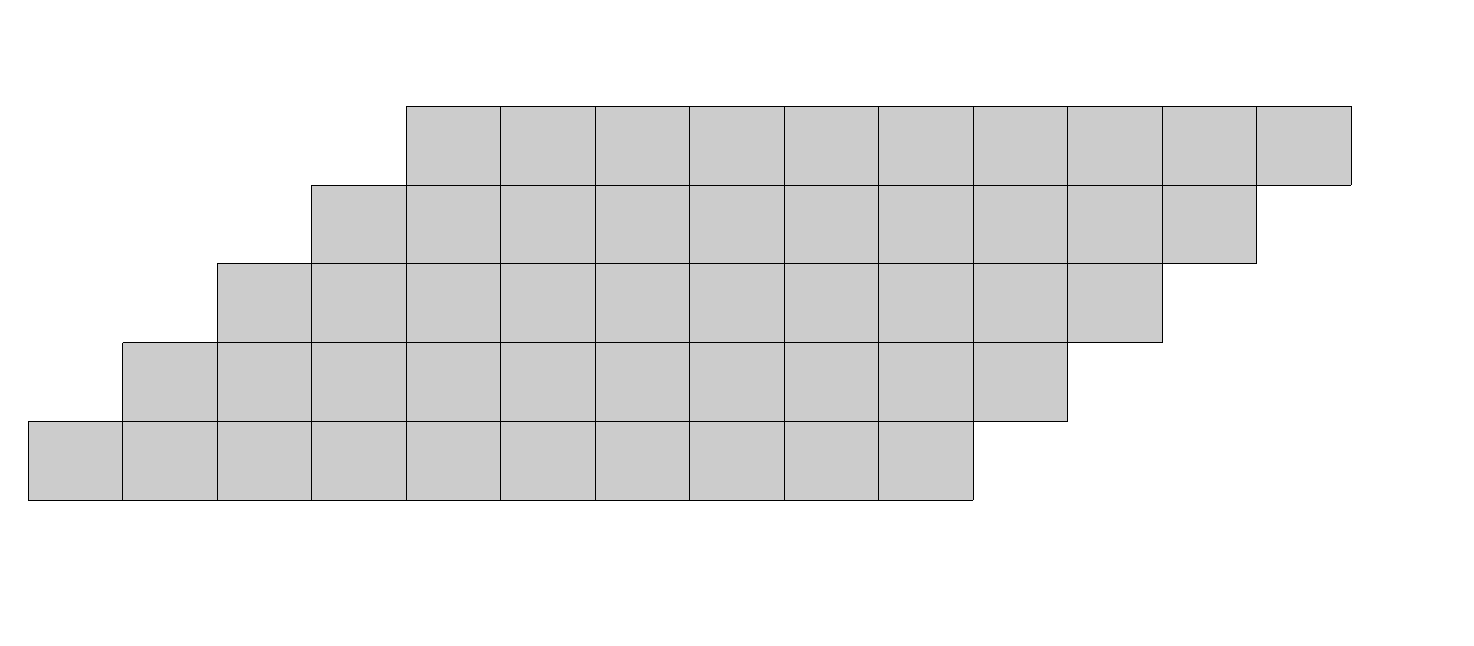
\begin{tikzpicture}[>=Latex]
    \path (0,-1.5) rectangle (18,6);
    \path[fill=gray1] (0,0)--++(12,0)--++(0,1)--++(1.2,0)--++(0,1)--++(1.2,0)--++(0,1)--++(1.2,0)--++(0,1)--++(1.2,0)--++(0,1)--++(-12,0)--++(0,-1)--++(-1.2,0)--++(0,-1)--++(-1.2,0)--++(0,-1)--++(-1.2,0)--++(0,-1)--++(-1.2,0)--cycle;
    \draw (0,0) --++ (0,1);
    \draw (1.2,0) --++ (0,2);
    \draw (2.4,0) --++ (0,3);
    \draw (3.6,0) --++ (0,4);
    \draw (4.8,0) --++ (0,5);
    \draw (13.2,5) --++ (0,-4);
    \draw (14.4,5) --++ (0,-3);
    \draw (15.6,5) --++ (0,-2);
    \draw (16.8,5) --++ (0,-1);
    \foreach \x in {4,...,10}{
      \draw (\x*1.2,0) --++ (0,5);
    }
    \draw (0,0)--++(12,0);
    \foreach \x in {0,...,3}{
      \draw (1.2*\x,\x+1) --++ (13.2,0);
    }
    \draw (4.8,5)--++(12,0);

  \end{tikzpicture}
\end{document}